
\section{Introduction}


% Magnetic microscopy has seen rapid technological advances, allowing measurements increasingly closer to the sample surface. In such proximity, the assumption that magnetic sources can be represented as pure dipoles becomes inadequate. Higher-order multipole terms, such as quadrupoles and octupoles, become relevant for accurate modeling. Existing methods based on spherical harmonic expansion can model these terms but require detailed knowledge of the source's size and shape, often acquired through tomography. However, this information is frequently unavailable due to the non-uniqueness of the magnetic inversion problem.

% Unlike gravitational potential data, where the center of mass provides a natural reference point for spherical harmonic expansion, magnetic data lacks an equivalent ``magnetic center''. This absence poses a challenge for applying spherical harmonic expansions to magnetic fields, particularly when the source geometry is unknown or irregular. In this context, we propose an alternative approach based on low-order multipole estimation that circumvents the need for spherical harmonic decomposition. By employing Euler deconvolution, we can estimate the central position of the magnetic source. This estimated center serves as a reference for computing magnetic multipole moments without requiring detailed knowledge of the particle's true shape or size, offering a more practical and computationally efficient strategy for analyzing complex magnetic field data.

% We propose a method that bypasses these limitations by estimating multipole moments using a Cartesian framework. The method requires only the center position of the source, as obtained via Euler deconvolution, and does not depend on spherical harmonics or source geometry. The objective of this paper is to implement and validate this Cartesian multipole fitting approach using synthetic data. We compare its performance with traditional dipole fitting methods and assess its advantages in modeling higher-order magnetic signals.


Magnetic microscopy continues will continue to push toward smaller sensor–sample standoff and higher spatial resolution, revealing complex magnetic behavior beyond dipole-dominated signatures. In these conditions, higher-order contributions (quadrupole, octupole, and beyond) become non-negligible \citep[\textit{e.g.,}][]{CortesOrtuno2021, CortesOrtuno2022,Bellon2025b}, particularly for larger grains, clustered sources, and measurements close to the sample. Although the dipolar contribution can alone be used to efficiently describe the full magnetic moment of particle (source) \citep{Bellon2025b}, it is the non-dipolar components of a stray field that will carry a particle's domain-state signature \citep{Fabian2019,CortesOrtuno2022}. Spherical–harmonic (SH) expansions \citep{CortesOrtuno2022,Lima2023} provide a compact and rotation–friendly representation of such fields. A non-intersecting shell is virtually built to contain the magnetic source and, when this is  well-centered and conservatively truncated, the stray field magnetic fit on the shell can be reliably used to calculate the observed fields in arbitrary planes. In the context of magnetic microscopy, this means being able to use surface plane measurements --  e.g., the vertical component of the magnetic field of a thin-section acquired through a Quantum Diamond Microscope (QDM) -- to invert the magnetic moment of a given source using SH expansions. On planar data, however, SH performance is sensitive to the choice of expansion center and degree: loss of orthogonality on the plane, miscentering, and noise can couple coefficients across degrees and bias low–order terms.

Technically, this issue could be addressed by performing three-dimensional tomographic experiments to determine the position of every magnetic source within the subsurface of the sample, as is commonly done in micromagnetic tomography (MMT) \citep{DeGroot2021, Cortez-Ortuno-2024}. However, incorporating tomography into the experimental workflow introduces additional complexity: standoff computerized CT scans generally do not provide sufficient resolution to detect the smallest single-domain (SD) and single-vortex (SV) particles. Even when high-resolution techniques do succeed, they are often chemically or structurally unresolved (e.g., Focused Ion Beam tomography, \cite{Nikolaisen-2020,Hristo-2025}), or they must be restricted to very small areas (typically on the order of $\sim 20~\mu\mathrm{m}^2$), as is the case for ptychographic X-ray computed nanotomography \citep{Bellon-2024a}. An alternative approach is to rely solely on the observed magnetic data and invert only for the detected anomalies, representing each anomaly by a virtual source enclosed within a single shell centered on that anomaly. A central practical difficulty is the absence of a natural “magnetic center”: unlike gravity, there is no center-of-mass analogue that can be identified a priori to stabilize an expansion \citep{Lima2023}. When source geometry is unknown or irregular, even small centering errors redistribute spectral power and degrade estimates. This motivates a complementary strategy in which the center is estimated from the field itself and, around that center, a low–order model captures the dominant curvature without relying on spherical functions.

We pursue this strategy by seeding the center with a modified Euler deconvolution strategy \citep{Reid1990,Souza-Junior2024,Souza-Junior2025} and then fitting a Cartesian multipole (CM) model (dipole, quadrupole, octupole) about that center. The method requires only a center (no explicit size/shape assumptions), integrates naturally with gradient–based optimization, and is well conditioned for local, planar problems. In parallel, we implement the SH formulation following recent developments \citep{Lima2023} to provide a baseline that is spectrally complete and transferable across heights when the center and truncation are well chosen.  We apply this methodology to two synthetic datasets: one generated using our CM model, and another based on a set of idealized spherical, prolate, oblate, and cuboctahedral equidimensional particles that were micromagnetically modeled. We compared the Cartesian and SH approaches, quantified their sensitivity to centering and model order, and delineated the regimes in which each method is preferred as a function of sensor height, grain size and shape, source overlap, and noise level.



\section{Methods}



\subsubsection{Spherical–harmonic inversion of \texorpdfstring{$b_z$}{Bz}}

To compare our new CM fitting method with a conventional spherical-harmonic (SH) representation \citet{Lima2023}, we construct an SH expansion that reproduces the measured vertical field component $b_z$ on the observation surface.  An SH expansion is valid provided that all magnetic sources lie inside a reference sphere of radius $a$, regardless of their geometry or exact location.  However, the choice of expansion center $\mathbf{c}$ strongly influences the conditioning and accuracy of the fit. Here we propose an alternative and more flexible strategy to choose the expansion center based on Euler deconvolution solution for a source's location ($x_c$,$y_c$,$z_c$) with optional refinement.

For $r > a$, where $a$ denotes the radius of a reference spherical shell enclosing all magnetic sources, the scalar magnetic potential is expanded in real spherical harmonics of maximum degree $N$. Differentiation of the potential and projection onto the laboratory $z$ axis yields: 

\[
b_z(r,\theta,\phi)
=\mu_0 \sum_{n=1}^{N}\left(\frac{a}{r}\right)^{n+2}
\sum_{m=0}^{n}
\Big[(n+1)\cos\theta\,P_{n}^{m}(\cos\theta)
+\sin\theta\,\partial_\theta P_{n}^{m}(\cos\theta)\Big]\,
\big(g_{n}^{m}\cos m\phi+h_{n}^{m}\sin m\phi\big).
\]

\noindent In this expression, $(r,\theta,\phi)$ are the spherical coordinates of the evaluation point, where  $r$ is the radial distance, $\theta$ the colatitude, and $\phi$ the azimuthal angle. The functions $P_n^{m}(\cos\theta)$ are the associated Legendre polynomials of degree $n$ and order $m$. The angular derivative $\partial_\theta P_n^{m}$ is evaluated in closed form via: 

\[
\partial_\theta P_{n}^{m}(\cos\theta)=
\frac{n\cos\theta\,P_{n}^{m}(\cos\theta)- (n+m)\,P_{n-1}^{m}(\cos\theta)}{\sin\theta}.
\]

We assemble a real design matrix $G$ whose columns correspond to the cosine- and sine-type basis functions associated with the coefficients $g_n^{m}$ and $h_n^{m}$ (with $h_n^{m}$ present for $m \ge 1$).  Each row of $G$ contains the evaluation of these basis functions at a particular observation point, as dictated by the expression for $b_z(r,\theta,\phi)$ above. The coefficient vector is then obtained through a standard linear least-squares solution.

The reference radius is set to $a = \max_i r_i$, where $r_i = \|\mathbf{x}_i - \mathbf{p}\|$ is the distance from the initial expansion center (obtained from Euler Deconvolution) to the $i$-th observation point. When needed, we refine the expansion center $\mathbf{c}$ by minimizing the RMS prediction error using a derivative-free search method \citep[Nelder–Mead,][]{Nelder-Mead1965}. At each candidate center, the spherical coordinates $(r,\theta,\phi)$ of all data points are recomputed, the design matrix $G$ is rebuilt, and the coefficients are re-estimated. This optional refinement is more computationally demanding, but it substantially improves stability and accuracy when the sources are clustered or asymmetric.




\subsection{Micromagnetically constrained dataset}

We obtained a variety of domain-states, in a way that we observe a transition from single-domain (SD), to single-vortex (SV), up to multivortex (MV) as the particle sizes increase (\hl{see Supplementary Figure XX}). Our SH expansion fits, evaluated up to degree 11, produce coefficients that explain so well the observed micromagnetic predicted stray-field that residuals are pratically neglectable (see Figure \ref{fig:spherical-harmonic-fitting}, which gives confidence that $b_z$-maps we produced with these fits capture the natural decay of stray-fields robustly. 

\begin{figure}[tb!]
  \centering
  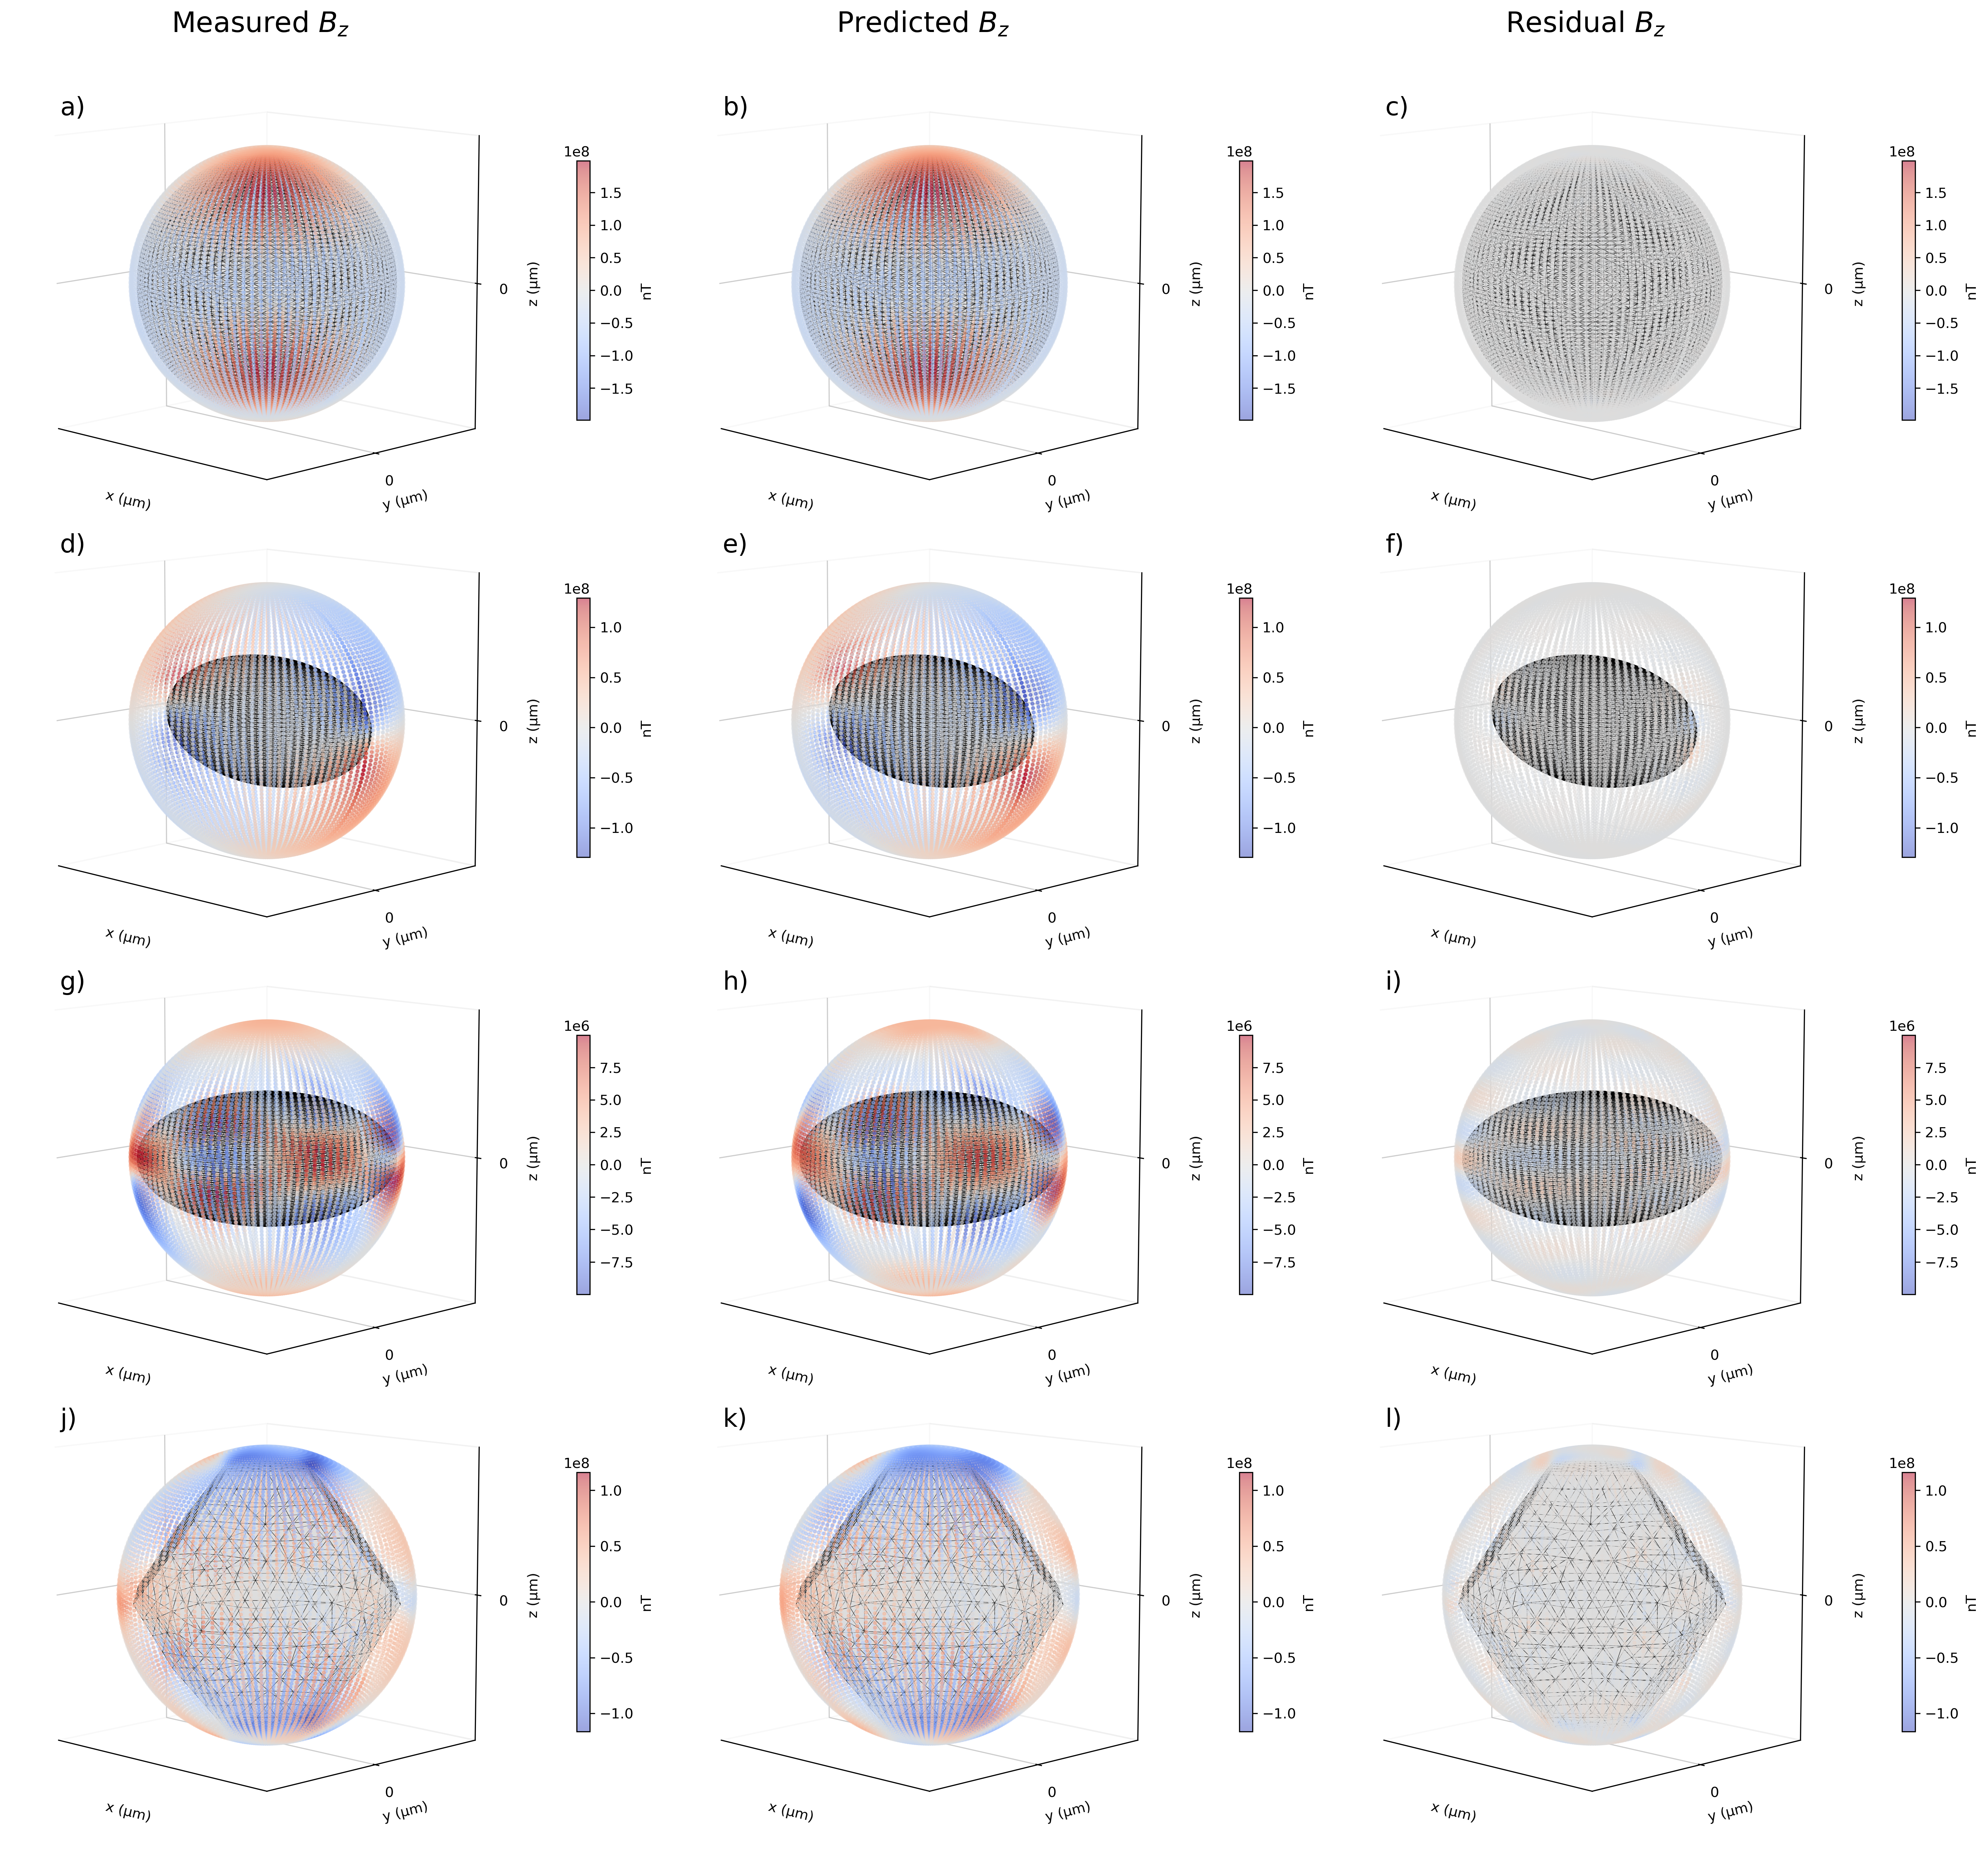
\includegraphics[width=1\linewidth]{paper/figures/particles_spherical_harmonic_fitting.png}
\caption{Micromagnetic forward models used for benchmarking. Columns show grain shape (sphere, prolate, oblate, euhedral); rows increase grain size. For each case, Merrill simulations produced $B_z$ on a spherical shell (left), the shell data were fit with real spherical–harmonic coefficients (middle: SH prediction on the same shell), and residuals are shown on the right. The close match indicates that the SH expansion faithfully represents the shell data across shapes and sizes.}

  \label{fig:spherical-harmonic-fitting}
\end{figure}

Before describing the comparison between our inversion results for this dataset, we first examined the influence of non-dipolar components as a function of distance by analyzing the power spectrum of each SH coefficient (Figure~\ref{fig:spherical-harmonic-spectro}). In all cases, the degree-1 term dominates the energy spectrum at all heights. For the smallest particles in the SD state (50 nm; Figure~\ref{fig:spherical-harmonic-spectro}a–d), it is effectively the sole contributor. A similar pattern is observed for SV states (100 nm; Figure~\ref{fig:spherical-harmonic-spectro}e–h): although the magnetic moments are arranged non-uniformly in a vortex, only the vortex core contributes significantly to the magnetization, resulting in an energy distribution across degrees that resembles the SD case. For more complex vortex states—those occurring in particles larger than 500 nm in our dataset—higher-degree terms become increasingly important as particle size grows. The larger the particle, the greater the height over which non-dipolar components remain relevant. For 500 nm particles, non-dipolar terms remain essential for achieving a good fit up to approximately \SI{1}{\micro\meter} above the sources (Figure~\ref{fig:spherical-harmonic-spectro}i–l). As particle sizes increase further, this threshold rises accordingly, typically to around 2–\SI{3}{\micro\meter}, and in some cases up to \SI{5}{\micro\meter} for oblate particles (Figure~\ref{fig:spherical-harmonic-spectro}o, s). These observation are consistent with those of \cite{Bellon2025b}, who evaluated this influence using solely fitting CM models in micromagnetically simulated stray-fields.  


\begin{figure}[tb!]
  \centering
  \includegraphics[width=1\linewidth]{paper/figures/fit_sphe_harm_in_different_heights.png}
\caption{Log-normalized spherical–harmonic power spectra on the shell for each shape (columns) and size (rows). Color indicates relative power per degree $n$ (warmer = higher). As grain size increases, power shifts from low degrees (dipole/quadrupole) toward higher degrees ($n\gtrsim 4$–6), especially impactful at small sensor heights. This spectral broadening explains the failure of finite-order multipole fits (e.g., octupole) for large grains near the sensor, while spherical harmonics remain accurate by capturing higher-order content.}

  \label{fig:spherical-harmonic-spectro}
\end{figure}


Fitting all the inversion routines to these non-noisy, micromagnetically coherent $b_z$ maps at different heights (Figure~\ref{fig:spherical-harmonic-model}) yields results that are fully consistent with the previous dataset. Both our new CM method (blue and black symbols) and the SH expansion using the Euler deconvolution method (pink symbols) (Figure~\ref{fig:spherical-harmonic-model}) outperform dipolar methods under all conditions. As before, dipolar fits degrade substantially for larger particles at close standoff distances; however, at sufficiently large distances, the dipolar-fit errors become smaller or at least approach the $5^\circ / 5\%$ level.


\begin{figure}[tb!]
  \centering
  \includegraphics[width=1\linewidth]{paper/figures/model_comparison_with_sphe_harm.png}
\caption{Planar $b_z$ predictions from the fitted spherical–harmonic models at multiple sensor heights (marker shapes) and grain sizes (colors), for sphere (a,e), prolate (b,f), oblate (c,g), and euhedral (d,h). Top row: angular misfit (degrees) between recovered and true dipole directions; bottom row: relative dipole-moment misfit (\%). Dashed gray lines mark practical targets (5$^\circ$ and 5\%). SH fits (magenta) maintain low misfits over the widest range of heights and sizes, whereas octupole models (green/black) deteriorate for larger grains at low $h$.}

  \label{fig:spherical-harmonic-model}
\end{figure}




\section{Discussions and Final Remarks}

\subsection{The applicability of Cartesian multipolar models}

Our CM model significantly improves field estimation near sources -- particularly when higher-order components significantly contribute to the signal --  when compared to purely dipolar fits. Unlike SH methods, ours does not rely on particle geometry, making it suitable for use when only center positions are known (or estimated), which perfectly fits a strategy that cannot rely on tomographic measurements to detect the source positions.

In our models, we do not analyze the effect of noise, as our goal is to provide a mathematical demonstration of the reliability of the proposed approach in generating multipolar sources in a phenomenological manner comparable to SH fitting. This equivalence is demonstrated in the final Results section, where we fit micromagnetically generated stray-field maps of SD, SV, and MV magnetic structures. The key difference between the two approaches—and the superior performance of SH at short sensor–sample distances—lies in the power-spectrum fitting (Fig.~\ref{fig:spherical-harmonic-spectro}). As grain size increases and the sensor approaches the sample, spectral energy shifts toward higher degrees ($n \gtrsim 4$–6), exceeding the span of an octupole. SH fitting naturally accommodates these higher-order terms and consistently projects them onto the measurement plane.

Yet, center choice is a primary control on performance. The position-error experiments (Figs.~\ref{fig:angular_misfit_position_error_comparison}--\ref{fig:moment_misfit_position_error_comparison}) show sharp minima in angular and moment misfits at zero error and symmetric growth with $|\Delta\mathbf{r}|$, with the steepest sensitivity along $\Delta z$. Initializing the expansion center with Euler deconvolution produces the minima near $\Delta\mathbf{r}\!\approx\!0$, and an optional Nelder–Mead refinement widens the basin of sub-degree (direction) and sub-percent (moment) accuracy, particularly for clustered or asymmetric sources.

In realistic scenarios, noise can be an important limitation when selecting an appropriate model. We have recently tested applications of the CM model \cite{Bellon2025b} using physically accurate QDM noise modeling and demonstrated that our inversion procedures are sufficiently robust to reliably predict the magnetic moment. However, we also showed that the rapid spatial decay of non-dipolar contributions, combined with measurement noise, can significantly limit the effectiveness of fitting higher-order multipolar components. In this aspect, for well-separated submicron sources at distances greater than $\approx \SI{2}{\micro\meter}$, a dipolar model has a similar performance. 

\subsection{Cartesian Multipole vs Euler deconvolution guided Spherical Harmonics expansion}

Multipole fitting, whether in Cartesian or spherical harmonic form, provide a more physically complete model for capturing the magnetic complexity of remanence carriers. They are especially useful when the goal is to resolve internal structures, account for multi-domain configurations, or interpret field curvature near the source. Their applicability is heightened when high-resolution maps show quadrupolar or higher-order features, or when dealing with non-uniform or clustered sources like silicate inclusions or magnetite aggregates.

One notable advantage of our CM model is its simplified implementation. Unlike spherical harmonics, which require special functions such as associated Legendre polynomials and demand careful handling of angular singularities, the Cartesian approach is more direct and can be implemented using standard vector calculus. This formulation also tends to exhibit improved numerical stability, particularly in local problems with planar geometries, since it avoids the singularities at the poles that are inherent in spherical coordinates. Furthermore, Cartesian multipole terms—such as dipole vectors and quadrupole or octupole tensors—correspond directly to physically interpretable quantities, which makes the inversion results more intuitive to analyze. Another benefit is the compatibility with modern optimization frameworks that support automatic differentiation. By expressing the field and its derivatives in Cartesian form, it becomes easier to integrate the model into open-source libraries like Magali/Fatiando a Terra, enabling gradient-based inversion and uncertainty quantification. Additionally, for highly localized sources such as those studied in magnetic microscopy, the Cartesian formulation is more efficient because it does not require a global coordinate system and allows for flexible modeling within confined spatial domains.

Despite these strengths, the Cartesian multipole expansion also presents some drawbacks. Unlike spherical harmonics, which form an orthonormal basis and thus promote parameter decoupling and inversion stability, Cartesian multipole tensors lack orthogonality. This can lead to stronger parameter correlations. Higher-order terms, such as quadrupole and octupole contributions, require symmetric, traceless tensors of increasing rank, which significantly increases the number of independent variables and adds to the implementation complexity. Besides -- for highly complex anomalies -- the number of Cartesian tensor components grows more rapidly than in the expansion order, raising the risk of overparameterization, which can be particularly problematic for underdetermined inverse problems.

Nonetheless, as shown, SH can be strongly sensitive the choice of coordinate origin. Even small shifts can substantially alter the higher-order terms, making the inversion more vulnerable to errors in source localization. 


%Tomographic multipole models, in particular, allow for nonparametric and flexible descriptions of the source distribution. They enable the estimation of continuous spatial variations in magnetization intensity and orientation, assist in identifying depth structure and internal features of extended sources when properly regularized, and support global inversions that integrate signals across entire scanned regions rather than focusing on isolated grains. Despite these strengths, applying tomographic multipole models to surface-acquired 2D magnetic data comes with several limitations. Most notably, the inversion problem is ill-posed and non-unique: magnetic fields measured over a surface do not uniquely determine the internal source configuration, making results highly sensitive to regularization and prone to a range of equivalent solutions. Truncating the expansion at a finite order can introduce edge effects and artificial oscillations, especially near scan boundaries. The inclusion of higher-order terms may also lead to overfitting noise or unresolved features, particularly in data with low signal-to-noise ratios. Computational complexity increases substantially as the number of expansion terms grows, demanding more time and memory. Furthermore, harmonic coefficients describe global properties of the field, making it difficult to localize individual grains—a significant drawback in densely packed samples. These challenges suggest that spherical harmonic-based tomographic models should be employed with caution, ideally supported by strong prior information or volumetric measurements that help constrain the inversion.





% \section{Discussion}

% Multipole models markedly improve field estimation near sources, especially when higher-order components are present, and they do so without assuming particle geometry—useful when only center positions are known. In magnetic microscopy, a pure dipole model remains attractive for isolated, nearly uniform grains at sensor heights large compared to grain size, or when the goal is rapid screening by total moment and orientation. Under these conditions, dipole inversion (aided by spatial priors like Euler deconvolution) is robust and fast. However, complex or aggregated sources, proximity to the sensor, and spatially structured residuals after dipole fitting expose the limits of the point-source assumption and can bias positions, directions, and intensities.

% Spherical harmonics and finite-order Cartesian multipoles provide a more complete description when the field exhibits curvature beyond dipolar. Our micromagnetic tests confirm that SH fits reproduce shell data with low residuals across shapes and sizes (Fig.~\ref{fig:spherical-harmonic-fitting}), and the same coefficients predict plane maps with high fidelity over a broad range of heights (Fig.~\ref{fig:spherical-harmonic-model}). In contrast, finite-order multipoles (e.g., octupole) degrade for larger grains at low heights. The shell power spectra (Fig.~\ref{fig:spherical-harmonic-spectro}) explain this breakdown: as grains grow and the sensor approaches the sample, spectral energy shifts toward higher degrees ($n\gtrsim4$–6) that exceed an octupole’s span, while SH accommodates these terms and projects them consistently to the plane.

% Center choice is a primary control on performance. The position-error experiments (Figs.~\ref{fig:angular_misfit_position_error_comparison}--\ref{fig:moment_misfit_position_error_comparison}) show sharp minima in angular and moment misfits at zero error and symmetric growth with $|\Delta\mathbf{r}|$, with the steepest sensitivity along $\Delta z$. Initializing the expansion center with Euler deconvolution produces the minima near $\Delta\mathbf{r}\!\approx\!0$, and an optional Nelder–Mead refinement widens the basin of sub-degree (direction) and sub-percent (moment) accuracy, particularly for clustered or asymmetric sources.

% Noise and model order introduce the usual bias–variance trade-off because planar coverage breaks SH orthogonality. We therefore select the smallest degree $N$ on the $R^2$ (or AIC/BIC) plateau and use weak Tikhonov damping; bootstrap medians with P16–P84 intervals reduce estimator skew under noise and outliers. Dipole and octupole fits are less variance-sensitive at large heights but become biased when unmodeled higher degrees are present; SH shows the opposite pattern—low bias when $N$ spans the spectrum, with variance controlled by conservative $N$ and mild damping.

% Practical guidance follows from these results. Use a dipole model when grains are isolated, $h/\text{grain size}\!\gtrsim\!5$, and residuals are unstructured. Use octupole when residual maps display clear quadrupolar curvature yet spectra remain compact ($n\!\lesssim\!3$). Prefer SH when grains are large or near the sensor, sources overlap, or plane-to-plane predictions are required; start from an Euler-based center and refine if misfits remain structured. For paleomagnetic applications, directional accuracy scales with both field strength and the number of resolved anomalies: strong fields ($\gtrsim10~\mu$T) need only a few hundred anomalies for unbiased directions, whereas weak fields demand substantially more and may be microscopy-limited. For paleointensity, bulk measurements approach but do not exactly recover the applied field even under favorable conditions, while SH-based inversions on magnetic images converge more closely—especially when using bootstrap medians—because spatially resolved data allow exclusion or down-weighting of altered or non-Arai grains.

% Limitations remain. Ill-posedness on planes, center sensitivity, and noise–variance trade-offs are fundamental constraints; truncation can introduce edge effects if $N$ is oversized, and coefficients are global descriptors that complicate grain-level attribution in dense assemblages. Future work should incorporate joint $(B_x,B_y,B_z)$ and multi-height data, physics-informed priors (e.g., micromagnetic texture or grain maps) to reduce non-uniqueness, automated center refinement, and adaptive degree selection to stabilize SH fits at scale.


%%%%%%%%%%%%%%%%%%%%%%%%%%%%%%%%%%%%%%%%%%%%%%%%%%%%%%%%%%%%%%%%%%%%%%%%%%%%%%%%%%%%%%%%%%%%%%%%%%%%%%%%%%%%%%%%%%%
% \section{Conclusion}
% We introduced a Cartesian multipole fitting method for magnetic microscopy that models higher-order magnetic signals without spherical harmonics or size/shape assumptions. Results on synthetic data demonstrate improved accuracy over traditional dipole fitting. Future work will apply the method to real datasets and explore further extensions.

% Using a Cartesian multipole expansion provides a viable and often advantageous alternative to spherical harmonics, especially in local or planar problems where physical interpretability, numerical stability, and implementation simplicity are prioritized. However, it comes at the cost of reduced orthogonality, increased parameter coupling, and greater sensitivity to coordinate choice. The decision between these formulations should be guided by the geometry of the problem, the available data coverage, and the specific goals of the inversion.

\section{Conclusions}

We presented and compared two complementary frameworks for modeling near-source magnetic fields in microscopy: a Cartesian multipole (CM) model and an adapted spherical–harmonic (SH) formulation. The Cartesian approach captures dipole, quadrupole, and octupole contributions through successive derivatives of the potential, requires no size/shape assumptions, integrates cleanly with gradient-based optimization, and offers highly interpretable parameters in local, planar settings. The SH approach expands the scalar potential in a complete basis by degree and order and projects consistently from enclosing shells to arbitrary planes, providing a natural spectral diagnostic of model adequacy.

Synthetic benchmarks and micromagnetic tests show clear regimes of preference. For isolated, nearly uniform grains at sensor heights large relative to grain size, dipole fits remain efficient and reliable. Finite-order Cartesian multipoles help when residual curvature is evident but the spectrum remains compact. For larger grains, overlapping sources, or small sensor heights—where shell spectra shift power to higher degrees ($n\gtrsim4$–6)—finite-order multipoles bias directions and moments, whereas SH fits remain accurate by accommodating the required degrees and transferring them robustly to measurement planes. Across all models, center choice is a primary control on performance: seeding the expansion center with Euler deconvolution and optionally refining it by RMS minimization yields sub-degree directional and sub-percent moment errors over the widest range of conditions.

These modeling and inversion frameworks improve the interpretive capability of micromagnetic analyses as spatial resolution increases and sensor–sample standoff distances are reduced. Higher-resolution field maps enhance higher-order spectral content and reveal source overlap that cannot be captured by dipole-only models. The combined use of Euler-centered initialization, optional center refinement, and conservative spherical-harmonic or Cartesian-multipole modeling provides a scalable and robust approach for incorporating this information while maintaining numerical stability.


%%%%%%%%%%%%%%%%%%%%%%%%%%%%%%%%%%%%%%%%%%%%%%%%%%%%%%%%%%%%%%%%%%%%%%%%%%%%%%%
\section{Open research}

The Python source code used to produce all results and figures presented here
is available at \url{https://github.com/\GitHubRepository} and
\url{https://doi.org/\ArchiveDOI} under the MIT open-source license.

Here we should cite all of the main software used, like Jupyter, numpy, scipy,
matplotlib, Fatiando, etc.

Cite any data sources as well.



%%%%%%%%%%%%%%%%%%%%%%%%%%%%%%%%%%%%%%%%%%%%%%%%%%%%%%%%%%%%%%%%%%%%%%%%%%%%%%%
\section{Acknowledgements}

We are indebted to the developers and maintainers of the open-source software
without which this work would not have been possible.
Acknowledge any non-author contributors to this study.
Statement about funding.

% Thank the editors and reviewers after review.
